\documentclass[a4paper, 16pt]{article}
\usepackage[top=3cm, bottom=3cm, left = 2cm, right = 2cm]{geometry} 
\geometry{a4paper} 
\usepackage[utf8]{inputenc}
\usepackage[portuguese]{babel}
\usepackage{textcomp}
\usepackage{graphicx} 
\usepackage{amsmath,amssymb}  
\usepackage{bm}  
\usepackage[pdftex,bookmarks,colorlinks,breaklinks]{hyperref} 
\hypersetup{linkcolor=blue,citecolor=blue,filecolor=black,urlcolor=black} 
\usepackage{memhfixc} 
\usepackage{float}
\usepackage{pdfsync}  
\usepackage{fancyhdr}
\usepackage[
backend=biber,
style=alphabetic,
sorting=ynt
]{biblatex}
\addbibresource{referencias.bib}
\pagestyle{fancy}

%\begin{document}
%\maketitle
\begin{document}

\title{%
  IF720- QUALIDADE DE SOFTWARE \\
  \large Relatório LaTeX para a disciplina de Introdução à Computação}


\author{Pierre Chevrollier Oriá}

\date{15 de Setembro de 2022}

\maketitle


\pagebreak

\section{Contexto}

\paragraph{Introdução}

\paragraph{}
Qualidade refere-se a um conceito subjetivo ligado à percepção de confiabilidade, segurança, acessibilidade e eficiência de um produto ou serviço. Qualidade de software, então, é a área que busca definir processos e padrões para o desenvolvimento de software capaz de produzir resultados corretos para os fins pretendidos, atuar dentro de determinados limites de tempo e infra-estrutura e, especialmente, atender às expectativas do cliente ou consumidor \cite{amlv}.



\begin{figure}[H]
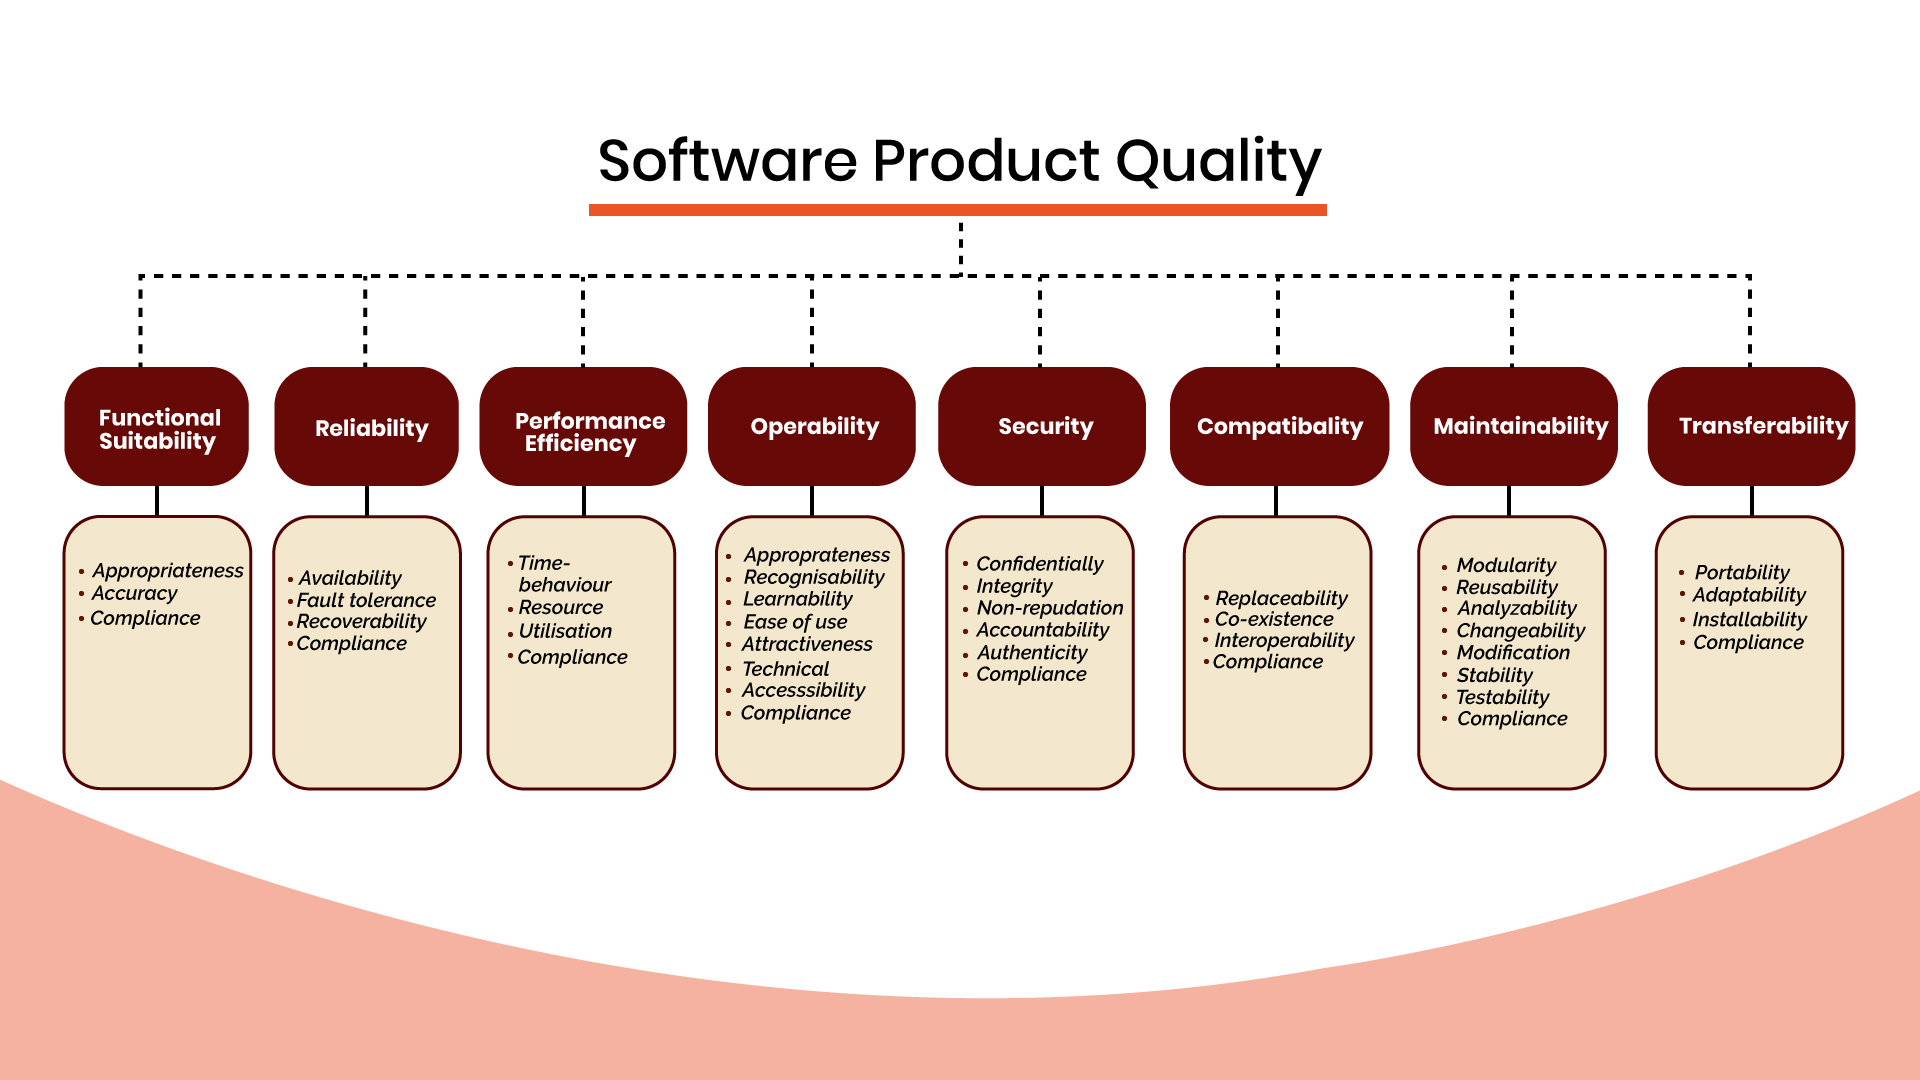
\includegraphics[width=15cm, height=10cm]{swqlt.jpg}
\centering
\caption{Qualidade de Software: elementos essenciais}
\cite{swq}
\end{figure}



\newpage

\paragraph{Relevância}

\paragraph{}
Dado o crescimento da digitalização de serviços na economia global \cite{digital}, duas implicações altamente relevantes surgem. A partir de uma perspectiva de consumidor de tecnologia, nos tornamos muito dependentes de software para navegar a vida cotidiana, a tal ponto que depositamos nossa confiança nele para gerenciar dados financeiros e pessoais extremamente sensíveis. Da parte do fornecedor, é esperado que seja entregue software confiável capaz de atuar em sistemas cada vez mais complexos e de alcançar ou superar um número crescente de competidores. Nesse contexto, torna-se essencial a criação de mecanismos para criação de software de excelente qualidade.

\paragraph{Relação com outras disciplinas}

\paragraph{}
Qualidade de Software está intimamente ligada à Engenharia de Software, visto que ambas tratam do desenvolvimento de código de forma macroscópica. Enquanto programação refere-se de forma mais restrita à criação de código, Engenharia e Qualidade de Software preocupam-se em estabelecer padrões confiáveis e escaláveis para criação de sistemas mais complexos, envolvendo colaboração entre múltiplos atores, respeito a normas técnicas e legais, gerenciamento de projetos e execução de testes intensivos.
Além de Engenharia de Software, a disciplina de Algoritmos também aborda uma questão central presente na área de Qualidade: a busca por códigos corretos e eficientes \cite{algoritmo}.


\pagebreak

\printbibliography

\end{document}

